\section*{Problema 1}
Solución de la ecuación de calor independiente del tiempo (Estado estacionario) por el método SOR
\begin{equation}
	\dv[2]{u}{x} + \dv[2]{u}{y} = 0. \label{calorperra}
\end{equation}
Con esto se tiene, que para un "grid" de $9\times 9$ de $1m^2$ y $100^oC$ en la frontera inferior e izquierda y $0^oC$ en la frontera superior y derecha, se tiene el siguiente mapa de calor.

\begin{figure}[H]
	\centering
	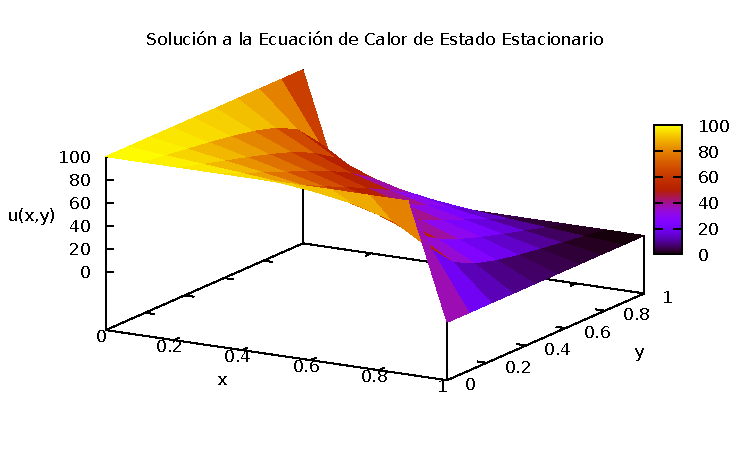
\includegraphics[scale=1]{../img/ej7-7.pdf}
	\caption{Mapa de calor de la solución a la ecuación \eqref{calorperra}.}
	\label{ej5-5}
\end{figure}



\begin{lstlisting}
// Librerias
#include <cmath>
#include <iostream>
#include <fstream>

using namespace std;



void output( ostream &of, double **u, double *x, double *y, int Nx, int Ny );
double p1( double x );
double p2( double x );
double q1( double y );
double q2( double y );




int main()
{
  int ITMAX = 10000; // maximo numero de iteraciones
  double eps = 1e-6; // tolerancia de error
  int Nx = 9;
  int Ny = 9; // grid
  double Lx = 1.0;
  double Ly = 1.0;
  double dx = Lx/Nx;
  double dy = dx;
  double alpha = 0.2; // factor para acelerar convergencia en SOR
  ofstream of( "solucion.dat", ios::out);


  // reservar memoria
  double *x        = new double[Nx+1];
  double *y        = new double[Nx+1];
  double **u       = new double*[Nx+1];
  double **u_nueva = new double*[Nx+1];

  for( int i=0; i<Nx+1; i++ ){
    u_nueva[i] = new double[Ny+1];
    u[i]       = new double[Ny+1];
  }


  // coordenadas
  for( int i=0; i<Nx+1; i++ ) x[i] = i*dx;
  for( int j=0; j<Ny+1; j++ ) y[j] = j*dy;


  // inicializar temperatura
  for( int i=0; i<Nx+1; i++ ){
    for( int j=0; j<Ny+1; j++ ){
      u[i][j]       = 0.0;
      u_nueva[i][j] = 0.0;
    }
  }


  // condiciones de frontera
  // lado inferior
  for( int i=0; i<Nx+1; i++ ) u[i][0]  = p1( x[i] );

  // lado superior
  for( int i=0; i<Nx+1; i++ ) u[i][Ny] = p2( x[i] );

  // lado izquierdo
  for( int j=0; j<Ny+1; j++ ) u[0][j]  = q1( y[j] );

  // lado derecho
  for( int j=0; j<Ny+1; j++ ) u[Nx][j] = q2( y[j] );


  // ciclo principal de SOR
  bool seguimos = true; // condicion de salida
  int k = 0; // numero de iteraciones


  cout << "Iniciando SOR" << endl;

  while( seguimos ){
    if ( k > ITMAX ){
      cerr << "Se alcanzo el numero maximo de iteraciones para SOR" << endl;
      exit(1);
    }

    seguimos = false;

    for( int i=1; i<Nx; i++ ){
      for( int j=1; j<Ny; j++ ){
	u_nueva[i][j] = 0.25 * ( u[i+1][j] + u[i-1][j] + u[i][j-1] + u[i][j+1] );

	// verificamos si seguimos o no
	if ( fabs( u_nueva[i][j] - u[i][j] ) > eps )
	  seguimos = true;

	// cambiamos iteraciones
	u[i][j] = u_nueva[i][j] + alpha*( u_nueva[i][j] - u[i][j] );
      }
    }

    // terminamos la iteracion
    k++;
  }


  cout << "SOR finalizo en " << k << " iteraciones" << endl;

  // escribir solucion
  output( of, u, x, y, Nx, Ny );


  return 0;
}




void output( ostream &of, double **u, double *x, double *y, int Nx, int Ny )
{
  for( int i=0; i<Nx+1; i++ ){
    for( int j=0; j<Ny+1; j++ )
      of << x[i] << "\t" << y[j] << "\t" << u[i][j] << endl;

    of << endl;
  }
}




double p1( double x ){ // Bottom edge
  return 100.0;
}

double p2( double x ){ // Top edge
  return 0.0;
}


double q1( double y ){ // Left edge
  return 100.0;
}

double q2( double y){ // Right edge
  return 0.0;
}
\end{lstlisting}

























%%%%%%%